\documentclass[a4paper,11pt]{article} %Set the type and parameter of the file
%----------------------------Region to load the package------------------------------------
\usepackage{graphicx} % Required for inserting images
\usepackage{amsmath} % Package containing loads of math equations and symbols type
\usepackage{derivative}%Package help us use derivative symbol more easily
\usepackage{minted}
\usepackage{commath}
\usepackage{graphicx}%Package allows us to insert the graph


\title{Probability Homework2}
\author{110612025 Dunkun Wei}
\date{October 25 2024}

\begin{document}
\maketitle

\section{Problem1's solution}
\subsection{(a)}
Let A:=\{first digit sends '1'\}, B:=\{first digit is erased\}.If $P(A \cap B) = P(A)*P(B)$ established, then event A and B are independent. $P(A)=1-p$ $P(B)=(\epsilon_0*p)+(1-p)*\epsilon_1$ and $P(A \cap B) = P(A \mid B)*P(A) = \epsilon_1 * (1-p)$, then we bring the value in the independent condition:\\
$(1-p)*(p*\epsilon_0+(1-p)*\epsilon_1) = \epsilon_1*(1-p)$\\reorganize the equation and we'll get:\\
$=>(1-p)*(p*(\epsilon_0-\epsilon_1))=0$\\
So when 
\begin{enumerate}
    \item $p=1$
    \item $p=0$
    \item $\epsilon_0 = \epsilon_1$
\end{enumerate}
happen, event A and event B will be independent

\subsection{(b)}
Let C:={First bit is not delivered correctly}, if A and B are conditionally independent, then it should obey this equation:
\begin{equation*}
P(A \cap B \mid C) = P(A \mid C)*P(B \mid C)
\end{equation*}
$P(A \mid C) = \frac{P(A \cap C)}{P(C)}=\frac{P(C \mid A)*P(A)}{P(C)} = \frac{(\alpha_1+\epsilon_1)*(1-p)}{p*(\alpha_0+\epsilon_0)+(1-p)*(\alpha_1+\epsilon_1)}$\\
$P(B \mid C) = \frac{P(B \cap C)}{P(C)} = \frac{P(C \mid B)*P(B)}{P(C)} = \frac{p*\epsilon_0+ (1-p)*\epsilon_1}{p*(\alpha_0+\epsilon_0)+(1-p)*(\alpha_1+\epsilon_1)}$\\
$P(A \cap B \mid C) = \frac{P(A \cap B \cap C)}{P(C)}=\frac{P(C)*P(A \mid C)*P(B \mid A \cap C)}{P(C)}$, because of multiplication rule.
$P(A \cap B \mid C) = P(A \mid C)*\frac{\epsilon_1}{\alpha_1 + \epsilon_1}$, since $P(A \cap B \mid C) \neq P(A \mid C)*P(B \mid C)$,A and B aren't conditionally independent.

\subsection{(C)}
Let $A_1$:=\{first digit sends '0'\}, $A_2$:=\{first digit sends'1'\}, $B_1$:={transmitted bit is delivered correctly}\\
By the total probability Theory:
\begin{align*}
    P(B_1) &= P(A_1 \cap B_1)+P(A_2 \cap B_1)\\
           &= P(B_1 \mid A_1)* P(A_1)+P(B_1 \mid A_2) * P(A_2)\\
           &= (1 - \epsilon_0 - \alpha_0)*p+(1- \epsilon_1 -\alpha_1)*(1-p)
\end{align*}

\section{Problem2's solution}
\subsection{(a)}
Assume X :=\{The amounts of '1' transmission\}, Y:=\{The amounts of '0' transmission\}\\
Let $Z:=$\{Total amount of the transmission\} = $X+Y$, and from the question, we know Z $\sim$ $Poisson(\lambda, T)$\\
$P(X=n) = \sum_{m=0}^{\infty}P(X=n,Y=m)$\\
By multiplication rule:\\
\begin{equation}
\label{equation1}
P(X=n,Y=m) = P(Z=n+m)*P(x=n \mid Z=n+m)
\end{equation}
$P(Z=n+m)$ $\sim Poisson(\lambda, T)$ $=\frac{e^{-\lambda T}*(\lambda T)^{m+n}}{(n+m)!}$\\
$P(X=n \mid Z=n+m)$ $\sim Binomial(n+m,p)$ and win n times \\$=C_{n}^{n+m}*p^n*(1-p)^m$\\
By \eqref{equation1},we have
\begin{align*}
    P(X=n) &=\sum_{m=0}^{\infty} \frac{e^{-\lambda T}*(\lambda T)^{m+n}}{(n+m)!}*C_{n}^{n+m}*P^n*(1-p)^m\\
           &= \frac{e^{\lambda T}*(\lambda T)^n *p^n}{n!} * \sum_{m=0}^{\infty}\frac{(\lambda T)^m*(1-p)^m}{m!}
\end{align*}
By the definition of $e^x$, $\sum_{m=0}^{\infty}\frac{(\lambda T)^m*(1-p)^m}{m!} = e^{\lambda T(1-p)}$\\
So $P(X=n) = \frac{e^{\lambda pT}*(\lambda PT)^n}{n!}$ $\sim$ $Poisson(\lambda p, T)$

\subsection{(b)}
Key idea of this problem is that we first calculate $CDF$ and then $P(X=k) = F_X(k)- F_X(k-1)$\\
$X_1$,$X_2$,\dots,$X_n$ $\sim$ $Geometric(p)$, $X=\max\{X_1,X_2,\dots,X_n\}$, $Y=\min \{X_1,X_2,\dots,X_n\}$\\
$CDF$ of X:\\
By definition :$F_X(k)=P_X(X \leq k)$, that means for all $i=[1,n]$, $X_i \leq k$\\
Since all the $X_i$ are independent, $F_X = F_{X_1} * F_{X_2} * \dots * F_{X_n}$\\
$CDF$ of Geometric: $P(X \leq k)=1 - P(X>k) = 1- \sum_{m=k+1}^{\infty}(1-p)^{m}*p=1-(1-p)^k$\\
Hence $F_X(k)=(1-(1-p)^k)^n$\\ 
$PMF$ of X:\\
$P_X(X=k)=F_X(k)-F_X(k-1)=(1-(1-p)^k)^n-(1-(1-p)^{k-1})^n$\\
$CDF$ of Y:\\
$F_Y(k)=P_Y(Y \leq K)$, that means at least one $X_i$ is smaller or equal to k .Use complementary rule, $P_Y(Y \leq k) = 1-P_Y(Y>k)$, $P_Y(Y>k)$ means for all $X_i$ is larger than k.\\
$P_Y(Y>k)=P_{X_1}(X_1>k)*\dots *P_{X_n}(X_n>k)$, and $P_{X_i}(X_i>k)=\sum_{m=k+1}^{\infty}(1-p)^m*p=(1-p)^k$\\
Hence, $F_Y(k)=(1-(1-p)^{kn})$\\
$PMF$ of Y:\\
$P_Y(Y=k)=F_Y(k)-F_Y(k-1)=(1-(1-p)^{kn})-(1-(1-p)^{n(k-1)})\\=(1-p)^{n(k-1)}*(1-(1-P)^n)$\\
,and $P_Y(Y=k)$ $\sim$ $Geometric(1-(1-p)^{n})$

\subsection{(c)}
Let $X_{S_2}$:=\{The amounts of T in whole 123 position\}, it can be seen as Binomial random variable, success probability is $P_T$, and failure probability is $P_A+P_C+P_G$.\\
$P_{S_2}(X_{S_2}=k)=\begin{cases}
    C_{k}^{123}*(P_T)^k*(P_A+P_C+P_T)^{123-k},&\text{if k=0,1,\dots,123}\\
    0,&\text{else}
\end{cases}
$
\section{Problem3's solution}
Let $X=\{1,2,3,\dots ,n\}$ and $H(X):=-\sum_{i=1}^{n}p_i*\ln p_i$
\subsection{(a)}
$H(\frac{1}{2}, \frac{1}{3}, \frac{1}{6})=-(\frac{1}{2}\ln \frac{1}{2}+\frac{1}{3}\ln \frac{1}{3}+\frac{1}{6}\ln \frac{1}{6})=\frac{2}{3} \ln 2+\frac{1}{2}\ln3$\\
$H(\frac{1}{2},\frac{1}{2})=\ln2$\\
$\frac{1}{2}*H(\frac{2}{3}, \frac{1}{3})=\frac{1}{2} \ln2 - \frac{1}{3} \ln3$\\
From above, we can prove that $H(\frac{1}{2}, \frac{1}{3}, \frac{1}{6})=H(\frac{1}{2},\frac{1}{2})+\frac{1}{2}*H(\frac{2}{3}, \frac{1}{3})$

\subsection{(b)}
\begin{figure}
    \centering
    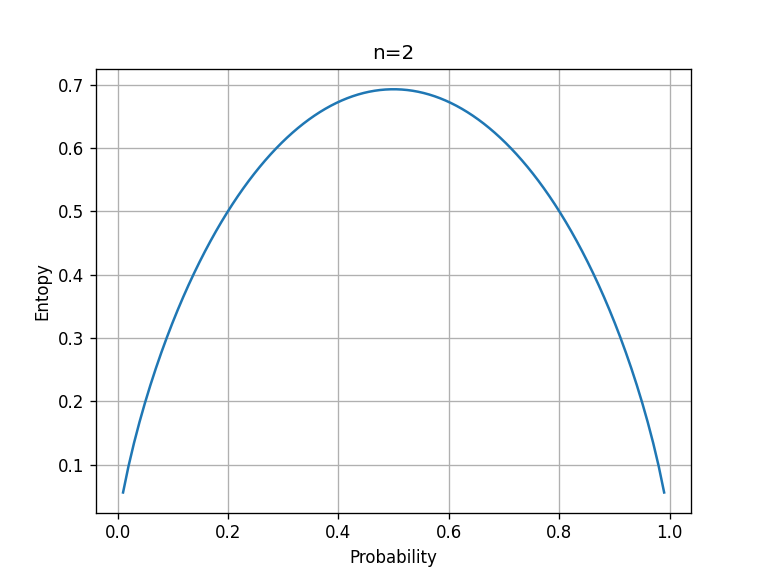
\includegraphics[width=0.7\linewidth]{figs/entropy_plot.png}
    \caption{probability vs entropy}
    \label{probability vs entropy}
\end{figure}
When $n=2$, $H(X)=-(p_1 \ln p_1 + (1-p)\ln (1-p))$.To find the $extremum$, take the derivative of $H(X)$\\
$\odv{H(X)}{p}=-(\ln p_1+1-\ln (1-p_1)-1)=0$,when $p_1= \frac{1}{2}$ have $extremum$, but don't know is maximum or minimum, so we take second derivative of $H(X)$ to find out.\\
$\odv[order=2]{H(X)}{p}=\frac{-1}{1-p_1}-\frac{1}{p}$,$0 \leq p$,so $\frac{-1}{1-p}-\frac{1}{p}$must smaller than 0, so $p=\frac{1}{2}$ is maximum, and $p=1$ or $p=0$ is minimum.\\
Maximum:$H(X)=\ln2$, when $p_1 = \frac{1}{2}$\\
Minimum:$H(X)=0$, when $p_1 = 1$ or $p_1=0$\\

\subsection{(c)}
Consider the case with $n \geq 2$.In this problem, we'll use the weighted inequality of arithmetic and geometric means:
\begin{equation}
\label{equation2}
    \frac{w_1x_1+w_2x_2+\dots+w_nx_n}{w} \geq (x_1^{w_1}*x_2^{w_2}*\dots *x_n^{w_n})^{\frac{1}{w}}
\end{equation}
where $w=w_1+w_2+\dots+w_n$\\
Let $w_i=p_i$ , $x_i = \frac{1}{p_i}$, and by axiom 1.:$w=1$
By \eqref{equation2}, use the value above,we have\\
$\frac{p_1\frac{1}{p_1}+\dots+p_n\frac{1}{p_n}}{1} \geq (\frac{1}{p_1}^{p_1}*\dots*\frac{1}{p_n}^{p_n})$\\
$=>n \geq (\frac{1}{p_1}^{p_1}*\dots*\frac{1}{p_n}^{p_n})$, and take $\ln$ on both side\\
$=>\ln n \geq -(p_1\ln p_1 + \dots +p_n\ln p_n)$,the maximum of $H(X)$ is $\ln n$\\
$PMF$ of $H(X)=\ln X$:
$PMF \{p_i\}_{i=1}^{n}=\begin{cases}
    \frac{1}{n},&\text{for i = 1,2,\dots ,n}\\
    0,&\text{else}
\end{cases}$
\subsection{(d)}
Find the minimum of the $H(X)$,using \eqref{equation2},let $w_i=p_i$, $x_i=\ln p_i$, and $w=1$,we get\\
$-(p_1\ln p_1+\dots+p_n\ln p_n)\geq (\ln p_1^{p_1}+\dots+\ln p_n^{p_n}) \geq 0$,so the minimum of $H(X)$ will be 0.In this situation:\\
$PMF \{p_i\}_{i=1}^{n}=\begin{cases}
    p_i=1,&\text{for any i=[1,n]}\\
    p_j=0,&\text{all j in [1,n] and $j \neq i$}  
\end{cases}$

\section{Problem4's solution}
\subsection{(a)}
(1.)E[X]\\
$X \sim Geometric(p)$, so $P_X(X=k)=(1-p)^{k-1}*p$, for $k=1,2,\dots ,\infty$\\
By definition\\
\begin{equation}
\label{equation3}
    E[X]=\sum_{k=1}^{\infty}k*P_X(X=k)
\end{equation}
By \eqref{equation3}, bring the value in it, and we'll get:\\
$E[X]=\sum_{k=1}^{\infty}k*(1-p)^{k-1}*p$, but it is hard to calculate this sum, instead we consider this equation:\\
$E_1[X]=\sum_{k=0}^{\infty}(1-p)^k=\frac{1}{p}$,and take derivative on both side.\\
$\odv{E_1[X]}{p}=\sum_{k=1}^{\infty}(-k)*(1-p)^{k-1}=\frac{-1}{p^2}$,and times -p on both side\\
$\sum_{k=1}^{\infty}k*p*(1-p)^{k-1}=E[X]=\frac{1}{p}$\\
(2.)$E[e^{tX}]$\\
By \eqref{equation3} and LOTUS, we can get:\\
\begin{align*}
    E[e^{tX}]&=\sum_{k=1}^{\infty}e^{tk}*P_X(X=k)\\
             &=(e^t*p)\sum_{k=1}^{\infty}(e^t(1-p))^{k-1}\\
             &=\frac{pe^t}{1-(e^t(1-p))}
\end{align*}
\subsection{b}
$z_n=(-1)^n\sqrt{n}$,for n=1,2,3,\dots,and $p_z(z_n)=\frac{6}{\pi n}^2$.\\
(1.)Var[X]\\
By definition:\\
\begin{equation}
\label{equation4}
    Var[X]=E[X^2]-(E[X])^2
\end{equation}
First find the value of $E[X^2]$,use \emph{Existance of momeny} to check whether it's exist or not.\\
\begin{align*}
    E[\abs{X^2}]&=\sum_{n=1}^{\infty}n*\frac{6}{(\pi n)^2}\\
                &=\sum_{n=1}^{\infty}\frac{6}{\pi^2 n}
\end{align*}
$E[\abs X^2]$will go to infinity because of the \emph{P-series test}, and by the \emph{Existance of the moment},$E[X^2]$ doesn't exist. So $Var[X]$ doesn't exist, too.\\
(2.)$\sum_{n=1}^{\infty}z_n^3*p_Z(Z_n)$\\
We can derive that $z_n^3=(-1)^n n^{\frac{3}{2}}$,bring the value into equation.\\
\begin{align*}
    \sum_{n=1}^{\infty}z_n^3*p_Z(Z_n)&=(-1)^n*n^{\frac{3}{2}}*\frac{6}{\pi^2n^2}\\
                                     &=\frac{6}{\pi^2}\sum_{n=1}^{\infty}(-1)^n*(\frac{1}{n^\frac{1}{2}})
\end{align*}
From \emph{Alternative Series test},\[ \lim_{n \to \infty} \frac{1}{n^{\frac{1}{2}}} = 0 \],
we can know that $\frac{6}{\pi^2}\sum_{n=1}^{\infty}(-1)^n*(\frac{1}{n^ \frac{1}{2}})$ converge,but $\frac{6}{\pi^2}\sum_{n=1}^{\infty}(\frac{1}{n^\frac{1}{2}})$is diverge due to \emph{P-series test}.\\
So by \emph{Riemann Rearrangement Series}, $\frac{6}{\pi^2}\sum_{n=1}^{\infty}(-1)^n*(\frac{1}{n^\frac{1}{2}})$ can be any number.\\
(3.)$E[Z^3]$\\
From(2.), we already know that $\sum_{n=1}^{\infty}\frac{6}{\pi^2n^{\frac{1}{2}}}$ is divergent due to \emph{P-series test}, so by \emph{Existance of moment}, $E[Z^3]$ doesn't exist.

\section{Problem5's solution}
\subsection{(a)}
The accuracy of the classifier with a 70\% /30\% partition of the dataset and a uniform prior is $0.979066985645933$\\
\subsection{(b)}
When we increase the prior from 0.1 to 0.5, the accuracy will improve, but when over the 0.5, the improvement became less significant, which shows that this model benefits from assuming high proportion of ham in dataset.\\
If we change the partition, we can see the consequence at $naive-bayes.ipynb$ file that when we near 0.1, the accuracy is very low due to the small training set, when we near 0.9, the accuracy become much better because of the more training. 








 




\end{document}
